\section{The Integration Algorithm}

The purpose of performing an intensity integration is 
to create a plot of average intensity as a function
of either $Q$, $2\theta$, or $\chi$. The algorithm
for performing an intensity integration is pretty
straight forward. In order to perform an intensity
integration, we must already know the calibration values
of the experiment for the particular image that will
be integrated. Than, a range and bin size for the
integration must be give. For example, you might
want to do a $Q-I$ integration from 2 to 5 with
100 bins. Whatever the range is, it 
must be specified before an integration is done.

The algorithm for performing the intensity integration
is as follows: loop over every pixel in the image. 
Add its intensity to the bin if it should be
in the bin based upon its value of $Q$, $2\theta$, or 
$\chi$. Remember that we need to use the calibration
values to calculate the corresponding $Q$, $2\theta$, and 
$\chi$ value using equations~\ref{ytermsydoubleprime}
\ref{xtermsxdoubleprime}, \ref{chitermsyx}, 
\ref{2thetatermsr}, and \ref{qterms2theta}.
After going through all the pixel, the bins then get averaged 
together. 

This program can constrain the integration. 
This means that you can perform, for example,
a $Q$ integration of only those pixels with some
particular range of $\chi$ values. Or, you can
constrain your $\chi$ integration to on a particular
$Q$ range. This could be used, for example, to
perform a $\chi$ integration of only a particular
diffraction peak. The algorithm for performing
the constraint isn't any more complicated. You just
only bin a particular intensity value if it is
allowed by the constraint.

Finally, the program can perform a polarization 
correction to the integration. The polarization 
correction formula is
\begin{align}
    I&=Im/PF \\ 
    PF&=P(1 - (\sin(2\theta)\sin(\chi-90))^2) + 
    (1 - P)(1 - (\sin(2\theta)\cos(\chi-90))^2)
\end{align}
with $Im$ the measured intensity. If this
is selected, what happens
then is that all pixels have their intensity
value corrected by this formula before they
are binned. Note that the $2\theta$ and $\chi$
values correspond to the particular value
that is being corrected.

\section{Integrating with the Program}


In order to perform a cake of the program you will have to 
already have loaded into the program one or more diffraction
data files and you will have to input calibration data
into the program. Figure~\ref{integration_page} shows the
\gui{Integrate} tab. This is where integration is done.
Notice that there are two separate inputs on the page. 
The input on the left is titled \gui{Q-I Integration}
and is for performing $Q$ integration.
The inputs on the left allow you to specify a
range in $Q$ that should be integrated.
The $Q$ range can be inputted with the
\gui{Q Lower?}, \gui{Q Upper?} inputs. The number of
bins in $Q$ space can be specified with the
\gui{Number of Q?} input. 
To perform a $Q$ integration, you have to push
the \gui{Integrate} button on the left.

\begin{SCfigure}[1][htb]
    \centering
    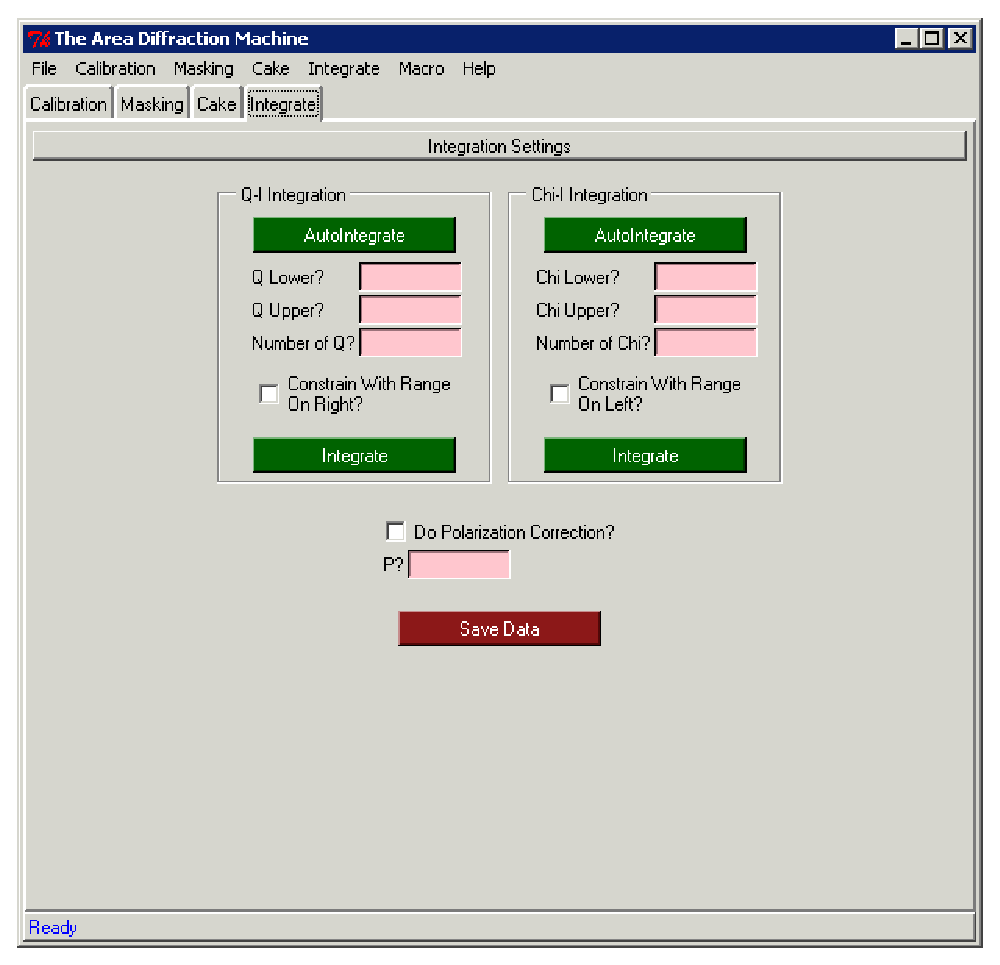
\includegraphics[scale=.75]{figures/integration_page.eps}
    \caption{A screen shot of the integration tab 
    to the program. This is the tab where you can 
    integrate data.} 
    \label{integration_page}
\end{SCfigure}

To perform a $\chi$ integration, you can use the inputs
on the right under the name \gui{Chi-I Integration}.
The inputs on the right allow you to specify
a range in $\chi$ with the \gui{Chi Lower?} and
\gui{Chi Upper?} inputs. The number of bins in
$\chi$ space can be specified with the
\gui{Number of Chi?} input. To perform the
$\chi$ integration, you have to push the
\gui{Integrate} button on the right.

\section{The Integration Window}

\begin{SCfigure}[1][htb]
    \centering
    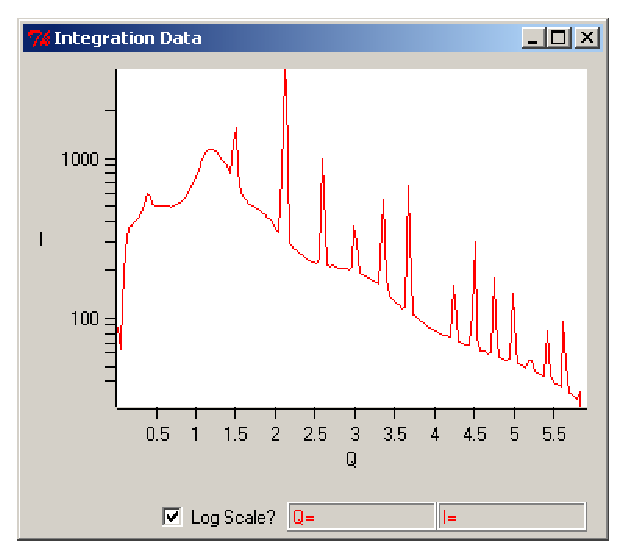
\includegraphics[scale=.75]{figures/integration_window_q.eps}
    \caption{A screen shot of the integration window that
    opens up after you perform an intensity integration.} 
    \label{integration_window_q}
\end{SCfigure}

\begin{SCfigure}[1][htb]
    \centering
    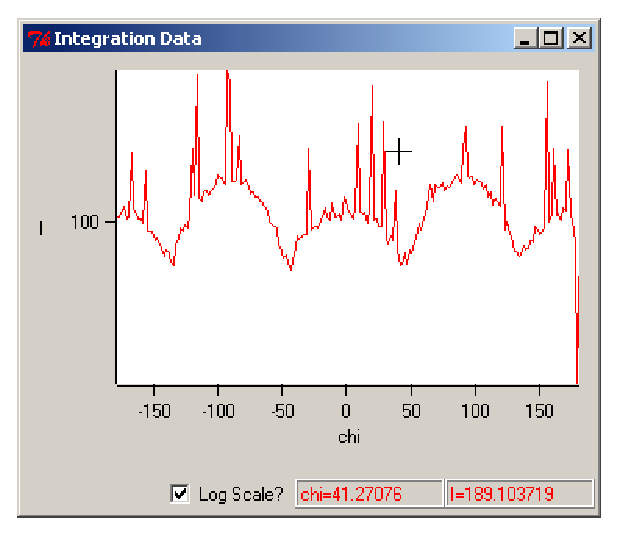
\includegraphics[scale=.75]{figures/integration_window_chi.eps}
    \caption{A screen shot of the integration window that
    opens up after you perform an intensity integration.} 
    \label{integration_window_chi}
\end{SCfigure}

After you push the integrate button, a line plot of the 
integrated data will be displayed in a new window. 
Figure~\ref{integration_window_q} shows 
the window displaying $Q$ integrated data
and figure~\ref{integration_window_chi} shows the
window displaying $\chi$ integrated ata.
Similar to the diffraction data display and the cake 
data display, this window has a couple of nice featuers
\begin{itemize}
    \item {\em Zoom into the data} - To zoom, left click
    on the data and hold down on the mouse. When you drag 
    the cursor, the program will create a resizing square. 
    When you let go of the mouse, the selected square will 
    be used as the outer bound and the image will be zoomed 
    into it. 
    \item {\em Zoom out of the data} - To unzoom, right
    click on the graph
    \item {\em Resize the window} - This will make the graph
    either larger or smaller. To do so, click on the bottom 
    right corner and drag. 
    \item {\em Read coordinates for a selected point} -
    When you mouse over the graph, the selected $Q$ (or $\chi$
    or $2\theta$) and intensity value will be displayed.
    \item {\em Log Scaling} - The \gui{Log Scale?} check box
    will toggle whether to display a log scale of the data.
\end{itemize}

\section{\texorpdfstring{Working in $2\theta$}{Working in 2theta}}

This program can integrate in $2\theta$ instead of $Q$. To 
do so, you have to go into menu bar up top and select
the \gui{Work in 2theta} option instead of the
\gui{Work in Q} option. Once you do this, the whole program
will just act like it was set to work in $2\theta$ all
along. The labels
on the program will change so that the option will say
\gui{2$\theta$-I Integration}. The other inputs will change
to \gui{2$\theta$ Lower}, \gui{2$\theta$ Upper}, and
\gui{Number of 2$\theta$}. When you push the left
\gui{Integrate} button, the program will integrate 
in $2\theta$ and the window that opens will show a plot
of average intensity as a function of $2\theta$.
If there are any values in the \gui{Q Lower} or
\gui{Q Upper}, they will be convert to $2\theta$
values when the program switches over. If you switch
from $2\theta$ back to $Q$, they will be converted
the other way.

\section{AutoIntegrate}

There is a convenience function similar to the
\gui{AutoCake} button called \gui{AutoIntegrate}. 
\gui{AutoIntegrate} will try to pick a nice range 
and then do the integration. The AutoIntegrate button 
on the left will guess at a nice range of $Q$ 
or $2\theta$ values and then do the $Q$ or
$2\theta$ integration.
It will always make the lower $Q$ or $2\theta$ 
value 0 and the upper value large enough
to include all the data.
It will set the number of $Q$ or $2\theta$ values to
200.

The \gui{AutoIntegrate} button on the right 
will guess a nice range of $\chi$ and then
do the $\chi$ integration. It will always 
set \gui{Chi Lower} to -180, \gui{Chi Upper} to
180, and \gui{Number of Chi} to 200.

\section{Constraining the Inputs}

As was described in the integration algorithm 
section, an integration in one parameter can 
be constrained by another parameter. For example,
a $Q$ or $2\theta$ integration can be done only 
of values in a particular $\chi$ range. Also,
A $\chi$ integration can be done only of a
particular $Q$ or $2\theta$ range. Of course,
it would be meaningless to constrain $Q$ by
$2\theta$.

To constrain the integration using the program,
there are two convenient 
\gui{Constrain With Range On Right?} and 
\gui{Constrain With Range On Left?} check boxes.
When you select
\gui{Constrain With Range On Right?}, the
$Q$ or $2\theta$ integration being done
will be constrained in $\chi$ by range
set with \gui{Chi Lower} and \gui{Chi Upper}.
When you select
\gui{Constrain With Range On Left?}, the
$\chi$ integration will be constrained by
either $Q$ or $2\theta$ (whichever mode the
program is currently in) by the lower and
upper inputs to the left.

\section{Masking}

The program can allows for masking of certain
pixels inside the image. 
Masking of intensity integrated data will be done
whenver the
\gui{Do Greater Than Mask?}, \gui{Do Less Than Mask?},
or \gui{Do Polygon Mask?} check boxes are selected.
Whenever the program finds an intensity value
that you specify should be masked (either because it 
is too large, too small, or in a polygon mask), it makes
sure not to bin that pixel and acts as though
it does not exist. So if you don't want to include
in your integration any values too large or too
small, you can use a threshold mask. If you
don't want to mask any values inside of a certain
region, you can use a polygon mask. 
Refer to Chapter \ref{pixel_masking} for information 
about how to apply a pixel mask.

\section{Saving Integrated Data}

After you have pushed the \gui{Integrate} buton
and performed a $Q$, $2\theta$, or $\chi$ integration,
you can save out the intensity integrated data
using the \gui{Save Data} button. The format of 
an intensity integration data file is as follows:
\begin{lstlisting}[caption={'A Cake Data File'}]
# Q vs I Intensity Integration
# Intensity integration of: C:/data/LaB6_14_02_56.mar3450 
# Data Integrated on Fri Mar 21 17:59:16 2008
# Calibration data used:
#   x center:    1725.0000000 pixels
#   y center:    1725.0000000 pixels
#   distance:     125.2960000 mm
#   energy:     12735.3957721 eV
#   alpha:          0.0000000 degrees
#   beta:           0.0000000 degrees
#   rotation:       0.0000000 degrees
#   pixel length:     100.0000000 microns
#   pixel height:     100.0000000 microns
# A polarization correction was applied
#   P = 1.000000
# A greater than mask was applied
#   Greater than mask = 10000.000000 (All pixels above 10000.000000 were ignored)
# A Less Than Mask was applied.
#   Less than mask = 50.000000 (All pixels below 50.000000 were ignored)
# Polygon mask(s) were applied
# Polygon(s) used in the analysis:
#   647.844364937	1369.72808587
#   1449.93738819	3226.88193202
#   2535.84794275	1449.93738819
#
#   1258.66905188	641.674418605
#   1215.47942755	999.531305903
#   1505.46690519	1116.76028623
#   1653.54561717	777.413237925
# Integration performed with a chi constraint
#   chi constraint lower: 90.000000
#   chi constraint upper: 270.000000
# Integration Range:
#   Q Lower = 0.000000
#   Q Upper = 6.726544
#   Number of Q = 200.000000
#   Q Step = 0.033633
# Q	Avg Intensity
0.016901	0.000000
0.050703	0.000000
0.084504	0.000000
0.118306	0.000000
0.152108	0.000000
0.185910	0.000000
...
\end{lstlisting}
The header is a bunch of lines that begin with \#.
Each line says something useful about the state
of the program when the integratinon was
done. 
If you perform an intensity integration in $\chi$
space instead, the header file will say
\macroline{\# Chi vs I Intensity Integration}
If two files were added together
and then integrated, the header file will say
\begin{lstlisting}[caption={'Alternate Header'}]
# Intensity integration of: C:/first.mar3450 C:/first.mar3450
\end{lstlisting}
Follwing the header string is the line
\macroline{\# Q Avg Intensity} (or \macroline{\# Chi Avg Intensity}
or \macroline{\# 2theta	Avg Intensity}). Following it is
the data. Each line contains one of the bins. The data
is tab seperated. The first number is the middle $Q$ (or
$\chi$ or $2\theta$ value) in the bin and the second number
is the average intensity.



